%************************************************
\chapter{Design and implementation}\label{ch:design}
%************************************************

%TODO resumir organización del capítulo





\section{Preliminaries about smart cards}


\subsection{Smart Card Communication Protocol}

To communicate the smart cards and the reader the ISO/IEC 7816-4 \citep{APDUISO} specifies a standardized protocol .

The messages, also kown as \acp{APDU}, are divided in APDU Commands and APDU Responses.

\textbf{APDU Commands} consist in 4 mandatory bytes (CLA, INS, P1, P2), and an optional payload.

\begin{itemize}
	\item CLA byte: Instruction class. Denotes if the command is interindustry standard or proprietary.
	\item INS byte: Instruction code. Indicates the specific command.
	\item P1, P2 bytes: Instruction parameters.
	\item Lc, 0-3 bytes: Command data length.
	\item Command data: Lc bytes of data.
	\item Le, 0-3 bytes: Expected response data length.
\end{itemize}

This way, minimal number of bytes are needed to transmit commands to the smart card, allowing manufacturer's personalization of the smart card behavior and capabilities along with standard operations.

\begin{figure}[bth]
	\begin{center}
		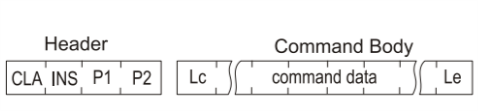
\includegraphics[width=0.55\linewidth]{gfx/APDUCommand}
	\end{center}
	\caption{APDU Command}
	\label{fig:APDUCommand}
\end{figure}


\textbf{APDU Responses} are generated inside the smart card, always as an answer to an APDU Command. They consist on an optional payload and two mandatory status bytes.


\begin{itemize}
	\item Response data: At most Le bytes of data.
	\item SW1-SW2 bytes: Status bytes. Encode the exit status of the instruction.
\end{itemize}

\begin{figure}[bth]
	\begin{center}
		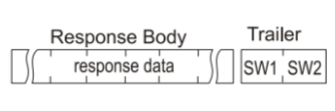
\includegraphics[width=0.55\linewidth]{gfx/APDUResponse}
	\end{center}
	\caption{APDU Response}
	\label{fig:APDUResponse}
\end{figure}




\hfil


The transmission protocol varies between different types of readers and smart cards (e.g. chip, contact-less), but what is common between every smart card interaction, is the \textit{APDU Command-Response Dialogue}. As long as the smart card has a power supply, it can maintain the memory in RAM between APDU Commands, what allows to do in two or more steps complex operations, transmit more bytes than a single APDU can admit, etc.

\hfil




\begin{figure}[bth]
	\begin{center}
		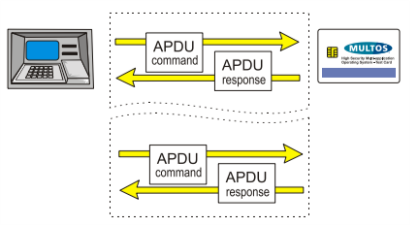
\includegraphics[width=0.75\linewidth]{gfx/APDUdialog}
	\end{center}
	\caption{APDU Command-Response Dialogue}
	\label{fig:APDUdialog}
\end{figure}

Originally, the Lc and Le bytes had only 1 byte, if present, restricting the payload data to be at most 256 bytes long. An extension to the protocol changed the meaning of a Lc or Le 0x00 byte (256 bytes long payload), so when the byte corresponding to Lc or Le started with 0x00, the next two bytes where the real length.  With this, an Extended APDU lets up to $65536$ bytes of data.

The problem here, is that not all readers or smart cards support extended APDUs. Originally, to send more than 256 bytes of data in an APDU Command, a \textit{Put Data} instruction is defined, so the smart card stores the payload in a buffer, until other APDU Command indicates how to use it.

To send more data in an APDU Response, the status bytes are set to: SW1=0x61 and SW2 to the remaining bytes to send. Because a smart card can't send APDU Commands, the card terminal must send a \textit{GET RESPONSE}, a special APDU Command, with Le set to the number of bytes specified in SW2. Iterating this process, the smart card can send as many bytes as it wants as Response.

With the introduction of Extended APDUs, this technique is no longer needed.






\subsection{MULTOS}

MULTOS is a multi-application smart card operative system, which provides a custom developing environment, with rich documentation \citep{MultosTechLib}. MULTOS smart cards communicate like any other smart card following the standard, but internally offers a very specific architecture, affecting the way one must code applications for it.

In this section we will present the main characteristics of a MULTOS smart card that shaped the ABC4Trust Card Lite code and that we had to be aware of when adapting it to IoT devices.

\paragraph{MULTOS programming languages} A native assembly language called MEL, C and, to a lesser extent, Java, are the available languages to code for MULTOS. In our case, ABC4T Card Lite uses MEL and C.

\paragraph{MULTOS Workflow}

Most of the transmission and communication process is done by MULTOS core, and it then selects, based on the CLA byte of the APDU, the application to load. This application is what most developers will only worry about, and is where their $main()$ function will start.

\begin{figure}[bth]
	\begin{center}
		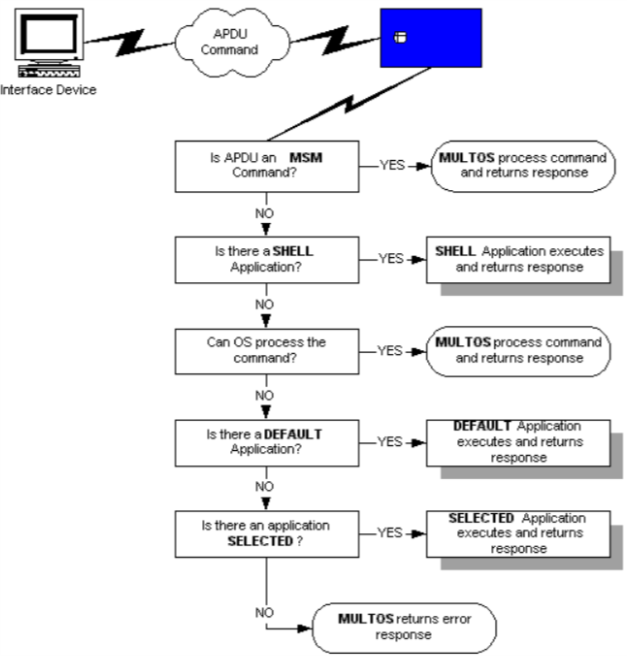
\includegraphics[width=\linewidth]{gfx/multosWorkflow}
	\end{center}
	\caption{MULTOS workflow}
	\label{fig:multosWorkflow}
\end{figure}

The application uses then the \textit{multos.h} file that declares multiple global variables already loaded with the needed data, including the APDU Command bytes.

Now the developer is in charge of checking what instruction was sent and if the APDU has the expected ISO Case. If everything is ok, code what needs to be run and write in specific data space the APDU Response bytes, call \textit{multosExit()} and MULTOS will be in charge to send the APDU Response.

In summary, our application starts with all data loaded and exits without worrying how to send the answer. A very comfortable workflow that we must now implement for our IoT device if we would want ABC4T Card Lite code to work.

\paragraph{MULTOS Memory Layout}

Each application in MULTOS has access to a specific memory layout, divided in different categories:

\begin{figure}[bth]
	\begin{center}
		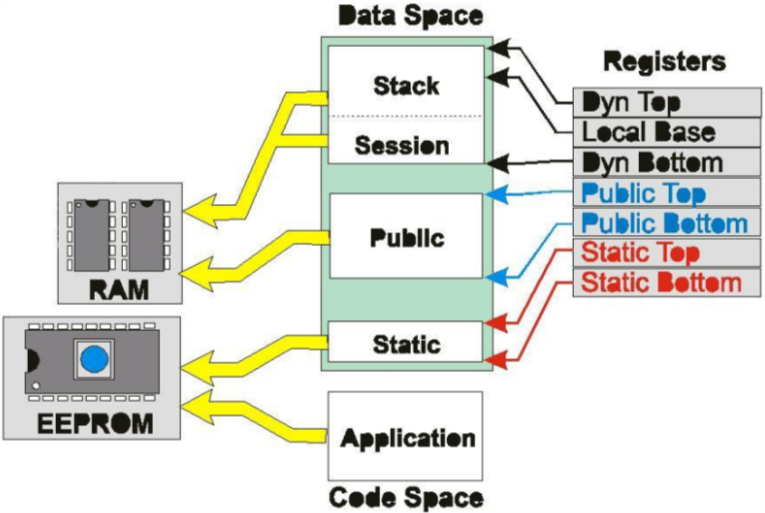
\includegraphics[width=\linewidth]{gfx/multosMemLay}
	\end{center}
	\caption{MULTOS Memory Layout}
	\label{fig:multosMemLay}
\end{figure}


The Code Space is where the application code is stored.
The Data Space is divided in Static memory, Public memory and Dynamic memory.

\textbf{Static memory} are the application variables declared after the specific \textit{\#pragma melstatic} compiler directive. These variables are stored in the non-volatile EEPROM, and any write is assured to be saved because they are not loaded into RAM.

\textbf{Public memory} can be seen as the input/output buffer for applications and MULTOS system. The APDU header appears at the top of Public, and command data at the bottom. The application writes then the APDU Response bytes in Public, at specific position (see \autoref{fig:multosPubMem}). To declare variables in this data space, the \textit{\#pragma melpublic} directive is available.

\textbf{Dynamic memory} works like usual program memory, with Session Data storing global variables and the Stack. The limited size of RAM in IoT devices and smart cards makes the use of dynamic memory not advisable. The compiler directive to use Session Data is \textit{\#pragma melsession}.


\begin{figure}[bth]
	\begin{center}
		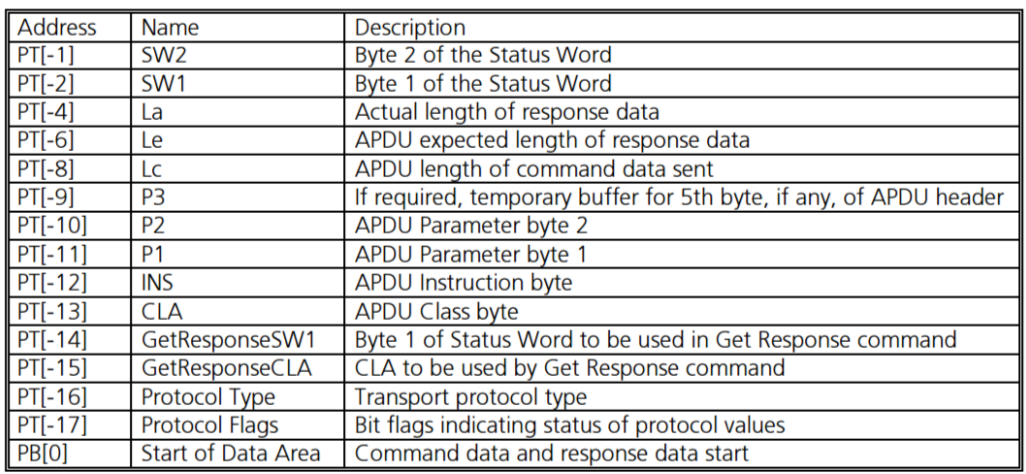
\includegraphics[width=\linewidth]{gfx/multosPubMem}
	\end{center}
	\caption{MULTOS Public Memory Data Map}
	\label{fig:multosPubMem}
\end{figure}


\hfil


With regards to primitive types, to avoid confusion with their sizes, MULTOS defines and uses the following data types specified in \autoref{fig:multosDataTypes}. It's important to notice that MULTOS is Big Endian
\marginpar{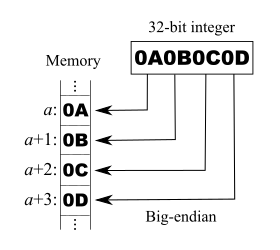
\includegraphics[width=\linewidth]{gfx/Big-Endian}\\Big-Endian, Wikipedia}
and when storing structures there is no padding between defined variables, unlike modern compilers that perform data structure alignment \citep{dataStructAlign} for performance.

\begin{figure}[bth]
	\begin{center}
		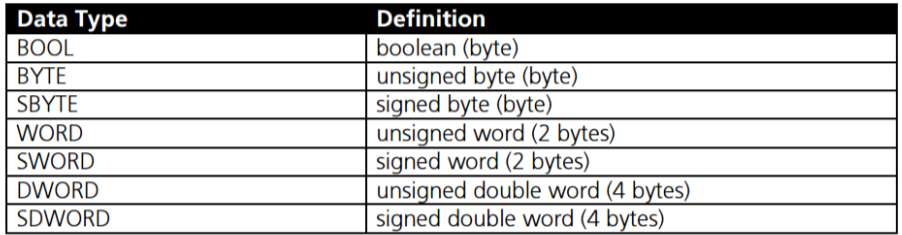
\includegraphics[width=\linewidth]{gfx/multosDataTypes}
	\end{center}
	\caption{MULTOS Data Types}
	\label{fig:multosDataTypes}
\end{figure}


\paragraph{MULTOS Standard C-API}

A collection of more than a hundred functions are provided for arithmetic, cryptography, memory and smart card operations. The \textit{multos.h} interface provides access to these functions, that ultimately call their respective primitive instructions in assembly code. The primitive instructions are but a system call with an operation code, loading data in the needed registers. Therefore,  no implementation for these tools is available, nor in C, nor in assembly code.

Nevertheless, the C-API documentation \citep{MultosTechLib} provides rich description for each function.



